\documentclass[12pt]{article}

\usepackage{fancyhdr}
\usepackage{amsthm}
\usepackage{amsmath}
\usepackage{graphicx}
\usepackage{amssymb}
\usepackage{esint}
\usepackage{subfigure}
\usepackage{color}
\usepackage{moreverb}
\usepackage{wrapfig}

\textwidth 17cm \topmargin -1cm \oddsidemargin 0cm \textheight 21.5cm
\pagestyle{empty} \pagestyle{fancyplain}
\lhead[\fancyplain{}{}]{\fancyplain{}{{\sc Adam Farnsworth:}}}
\chead[\fancyplain{}{}]{\fancyplain{}{{\sc Final}}}
\rhead[\fancyplain{}{}]{\fancyplain{}{{\sc Fall 2017}}}

\newcommand{\etal}{\textit{et al. }}

\begin{document}
\centerline{\Large\textbf{Final}}
\vspace{2cm}
\section{Problem 1}\label{sec::Problem 1}
\section*{Introduction}\label{sec::Intro}
The goal of this project is to determine the optimal time for boiling a potato.  To do this, I use the problem in two spatial dimensions and approximate the potato by a rectagle of size 4 cm by 5 cm.  At time $t_{start}=0$ a pan is filled with water containing the potato, and is placed on a stove top.  The potato and the water are at room temperature $T_{room} = 20^\circ C$.  The temperature of the water rises from $20^\circ c$ to $100^\circ c$ in 60 seconds and stays at $100^\circ C$ afterwards.  At the temperature of $65^\circ$ the cellular structure of the potato begins to change and the starch tarts to gelatinize.  Assimg that it takes 300 seconds for the potato's material to get fully cooked after it has reached $65^\circ C$  The temperature $T = T(t,x,y)$ inside the potato satisfies the heat diffusion equation below:
\begin{center}
$
\frac{\partial T}{\partial t}= \lambda \Delta T , (x,y) \in \Omega
$
\end{center}
with the boundary conditions:
\begin{center}
$
T(t,x,y) = T_{water}(t), (x,y) \in \partial \Omega
$
\end{center}
and the initial conditions
\begin{center}
$
T(0,x,y) = T_{room}(t), (x,y) \in \partial \Omega
$
\end{center}
where $\lambda$ is the thermal diffusivity of the potato's material, $\Omega$ and $\partial \Omega$ denote the domain in space occupied by the potato and the boundary of this domain.

simulate the flow around a rotating cylinder.  The two spatial directions domain is $\Omega = (x_L, x_R) X(t_B,Y_T)$ with a time interval of $[t_{start}, t_{final}]$, velocity vector $\overrightarrow{v} = \begin{bmatrix}
           v_x \\
          v_y \\
         \end{bmatrix}$ and a function $c = c(t,x,y)$ satisfying the advection equation below:\\
\begin{center}
$
\frac{\partial c}{\partial t} + \overrightarrow{v} \cdot \bigtriangledown c = f(t,x,y)$, for all $(x,y)$ $ \in$ $ \Omega$ and $ t$ $ \in$ $ [t_{start},t_{final}]$
\end{center}
with boundary conditions:\\
\begin{center}
$c(t,x,y) = g(t,x,y)$, for all $(x,y)$ $ \in$ $ \Omega$ and $ t$ $ \in$ $ [t_{start},t_{final}]$
\end{center}
where $\partial \Omega$ is the boundary of domain $\Omega$, and initial data:
\begin{center}
$c(t_{start},x,y) = c_{start}(x,y)$, for all $(x,y)$ $ \in$ $ \Omega$
\end{center}
where $f(t,x,y), g(t,x,y)$ and $c_{start}(x,y)$ are given functions.
\subsection{Part a}\label{sec::a}
The heat transfer in a rectagular domain $\Omega = [x_l;x_r]X[y_b;y_t]$

\begin{center}
$\begin{cases} 
\frac{\partial T}{\partial t} = -\lambda \Delta T + f, (x,y) \in \Omega  \\
T(t,x,y) = T_{bc}(t,x,y), (x,y) \in \partial \Omega  \\
T(t_{start},x,y) = T_{start}(t,x,y), (x,y) \in \Omega  \\
 \end{cases}$
\end{center}
where $\lambda$ is the thermal diffusivity of the material, $f=f(t,x,y), T_{bc}(t,x,y)$ and $T_{start}(x,y)$ are given functions describing the source term, boundary conditions and initial conditions.

Using the diffusion equation ath the moment of time $t_{tn+1}$ and location $(x_i, y_j)$ I get:
\begin{center}
$\frac{\partial c}{\partial t} (t_{n+1}, x_i,y_j) + D \frac{\partial ^2 c}{\partial x^2} (t_{n+1}, x_i,y_j) + D \frac{\partial ^2 c}{\partial y^2} (t_{n+1}, x_i,y_j) + f (t_{n+1}, x_i,y_j)$
\end{center}
and after using the backward finite difference formula to approximate the time derivitive, I can then approximate the spatial derivative in the x and y directions:
\begin{center}
$
\frac{\partial ^2 c}{\partial x^2} (t_{n+1}, x_i,y_j) \approx \frac{c(t_{n+1}, x_{i+1},y_j) - 2c(t_{n+1}, x_i,y_j)+c(t_{n+1}, x_{i-1},y_j)}{\Delta y^2}
$
\end{center}
\begin{center}
$
\frac{\partial ^2 c}{\partial y^2} (t_{n+1}, x_i,y_j) \approx \frac{c(t_{n+1}, x_{i},y_{j+1}) - 2c(t_{n+1}, x_i,y_j)+c(t_{n+1}, x_{i},y_{j-1})}{\Delta x^2}
$
\end{center}
using these I can obtain the expression:
\begin{center}
$
\frac{c_{i,j}^{n+1}-c_{i,j}^n}{\Delta t} = D \frac{c_{i+1,j}^{n+1}-2c_{i,j}^{n+1}+c_{i-1,j}^{n+1}}{\Delta x^2} + D \frac{c_{i,j+1}^{n+1}-2c_{i,j}^{n+1}+c_{i,j-1}^{n+1}}{\Delta y^2}+ f(t_{n+1}, x_i, y_j)
$
\end{center}
from here I can use this to directily apply to the problem to obtain:
\begin{center}
$
 f (t,x,y) = (2*D-1)*sin(x)*cos(y)*exp(-t)
$
\end{center}
\newpage
\subsection{Part b}\label{sec::b}
Implement the implicit scheme for this problem with the following example:

\begin{eqnarray}
\textrm{Domain:}\quad \quad \quad \quad \quad \quad \quad \quad \quad \Omega &=& [-1;1]X[-0.5;1.7]  \\\nonumber
\textrm{Thermal diffusivity: }\quad \quad \quad \quad \lambda &=& 0.75\\\nonumber
\textrm{Exact solution:}\quad \quad \quad \quad  \quad T_{exact}&=&sin(x)cos(y)exp(-t) \\\nonumber
\end{eqnarray}
where inital conditions $T_{start}(x,y)$, boundary conditions $T_{bc}(t,x,y)$ and source term $f(t,x,y)$ are calculated from the exact solution $T_{exact}$.  Solve the heat equation from $t_{start}=0$ to $t_{final}=1$ for grid resolutions $(N_x,N_y)=(25,30), (60,60)$ and $(100,120)$ with time step $\Delta t=0.5 \Delta x$.  Calculate errors of numerical solutions as the maximum absolute deviation from the exact solution at the moment of time $t=t_{final}$ and determine the order of accuracy of the numerical method.


\begin{table}[bht]
\centering

\begin{tabular}{|l|l|l|}
\hline
Matrix Size & Error        & Order of Accuracy \\ \hline
25 X 30     & 0            & 0                 \\ \hline
50 X 60     & 2.784527e-04 & 1.06844           \\ \hline
100 X 120   & 1.362070e-04 & 1.03163           \\ \hline
\end{tabular}
\caption{Errors and Order of accuracy}
\label{Problem 1b}
\end{table}

\newpage
\subsection{Part c}\label{sec::c}
Simulate the process of bliling a potato with the following parameters:

\begin{eqnarray}
\textrm{Domain:}\quad \quad \quad \quad \quad \quad \quad \quad \quad \Omega &=& [-2;2]X[-2.5;2.5] cm  \\\nonumber
\textrm{Thermal diffusivity: }\quad \quad \quad \quad \lambda &=& 0.0015 \frac{cm^2}{s}\\\nonumber
\textrm{Inital conditions:}\quad \quad \quad \quad  \quad T_{start}(x,y)&=&20^o  C\\\nonumber
\textrm{Boundary conditions:}\quad \quad \quad \quad  \quad T_{bc}(t,x,y)&=&min(20 + 80 \frac{t}{60},100)^o  C\\\nonumber
\textrm{Source term:}\quad \quad \quad \quad  \quad f(t,x,y)&=&0\\\nonumber
\end{eqnarray}
Solve the heat equation from $t_{start} = 0$s to $t_{final}=1500$s using $N_x = 80$ grid points in the x direction and $N_y = 100$ grid points in the y direction and time step $\Delta t = 5$s.  Plot the temperature at the center of the potato$((x,y) = (0,0))$ vs time and determine when this temperature reaches $T_{cooking}=65^o C$.  Add 300 seconds to the found time to obtain the total time needed to cook a potato.  Take snapshohts of the temerature distribuion inside the potato at moments of time $t = 0, 200, 400, 600$s

**see following page for solution**

\newpage
\begin{figure}[h]
\begin{center}
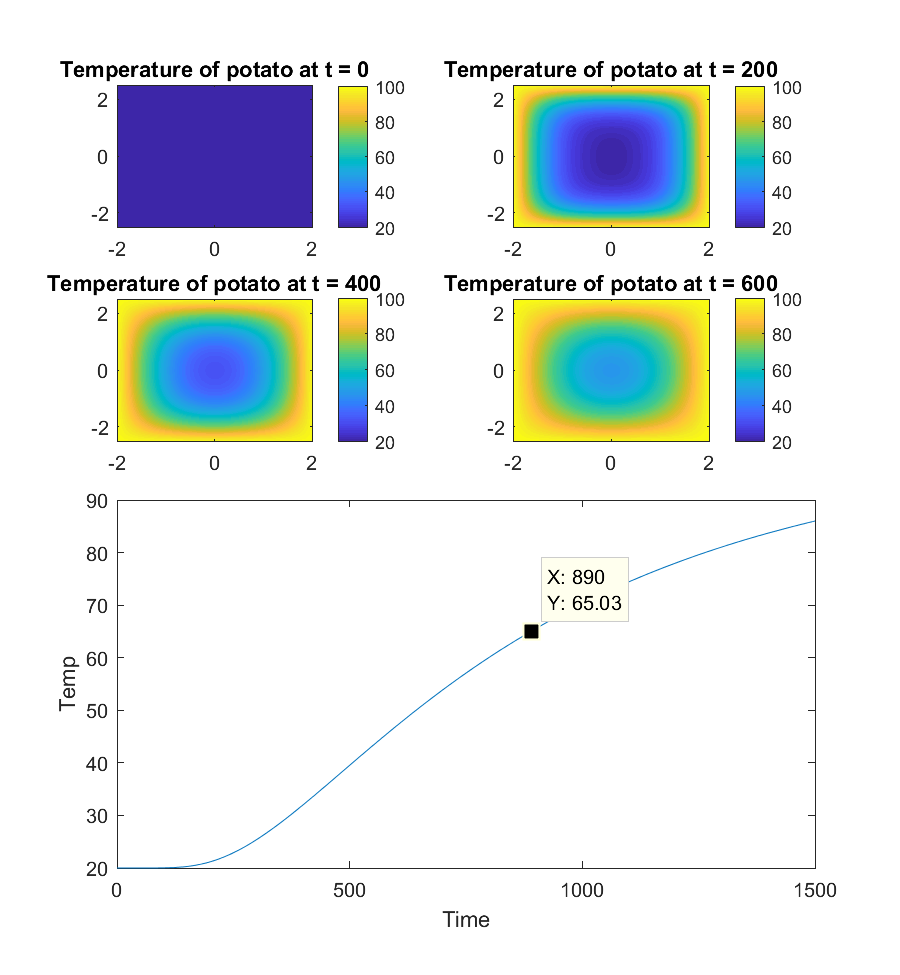
\includegraphics[width=.8\textwidth]{potato}
\end{center}
\caption{Simulation for potato} \label{fig::MyFigure}
\end{figure}

\newpage
\section{Problem 2}\label{sec::Problem 2}
\section*{Introduction}\label{sec::Intro}
The goal of this project is to estimate what beaches should be closed to the public after a oil spill occurs.  Its the day after a broken onshore pipeline near Santa Barbara spewed oil down a storm drain and into the ocean for several hours before it was shut off. Currents and natural diffusion of contaminants are two effects that account for how the oil spreads. In order to avoid unsafe bathing, the city of Santa Barbara has tasked you to estimate what beaches should be closed to the public. According to health officials, a beach where the concentration of oil is (strictly) greater than $c_{limit} = .006$ is deemed unsafe.  As an engineer, you model this process by an advection diffusion equation in two spatial demensions.  In addition, you assume that the stretch of the coast you are intered in is straight.  You thus consider a domain $\Omega = [x_l;x_r] X [y_b,y_t]$ a given velocity vector $\overrightarrow{v} = \begin{bmatrix}
           v_x \\
          v_y \\
         \end{bmatrix}$ representing the ocean's currents, a source term, $f = f(t,x,y)$ representing the amount of oil spilling into the ocean and concentration $c = c(t,x,y)$ representing the concentration of oil into the ocean.  The concentration thus satisfies the advection diffusion equation:
\begin{center}
$ \frac{\partial c }{\partial t} + \overrightarrow{v} \cdot \Delta c = D \Delta c + f$, for all $(x,y) \in \Omega$ 
\end{center}
where D is the rate of diffusion of oil in water, with the initial conditions $c(t_{start},x, y) = 0$.  Let us assume that the left, right and top boundaries of domain $\Omega$ are far enough, so that the oil concentraion stays zero at those boundaries during the course of simulation, that is, 
\begin{center}
$c(t,x,y) = 0, $ if $x = x_l, x = x_r, $ or $ y = y_t$
\end{center}
However, at the bottom boundary of the domain $\Omega$ the oil concentration has to satisfy the no flux condition
\begin{center}
$D \frac{\partial c}{\partial y} - v_y c = 0, $ if $ y = y_b$
\end{center}

\newpage
\subsection{Part a}\label{sec::a}
Consider a generalized advection diffusion problem in a rectangular domain $\Omega = [x_l;x_r] X [y_b;y_t]$

\begin{center}
$\begin{cases} 
\textrm{PDE:} \quad \quad \frac{\partial c}{\partial t} + \overrightarrow{v} \cdot \triangledown c = D \Delta c + f, \quad \quad(x,y) \in \Omega  \\
\textrm{BC:} \quad \quad c(t,x,y) = c_{bc}(t,x,y) \quad \quad\textrm{  if } x = x_l, x = x_r, \textrm{or } y=y_t \\
\quad \quad \quad \quad D \frac{\partial c}{\partial y} - v_y c = g(t,x,y) \quad \quad \textrm{ if } y = y_b \\
\textrm{IC:}\quad \quad c(t_{start}, x, y) = c_{start} (x,y), \quad \quad (x,y) \in \Omega \\

 \end{cases}$
\end{center}
where D is the diffusivity, $ f = f(t,x,y), c_{bc} = c_{bc}(t,x,y), g = g(t,x,y)$ and $c_{start} = c_{start}(x,y)$ are given functions describing the source temr, boundary conditional and initial conditions. 
Using similar logic to Problem 1 a) for the implicit approximation, I used the explicit upwind approximation by first using the diffusion equation at the moment of time $t_n$ at location $(x_i,y_j)$:
\begin{center}
$\frac{\partial c}{\partial t} (t_{n}, x_i,y_j) + D \frac{\partial ^2 c}{\partial x^2} (t_{n}, x_i,y_j) + D \frac{\partial ^2 c}{\partial y^2} (t_{n}, x_i,y_j) + f (t_{n}, x_i,y_j)$
\end{center}
and after using the forward finite difference formula to approximate the time derivitive, I can then approximate the spatial derivative in the x and y directions:
\begin{center}
$
\frac{\partial ^2 c}{\partial x^2} (t_{n}, x_i,y_j) \approx \frac{c(t_{n}, x_{i+1},y_j) - 2c(t_{n}, x_i,y_j)+c(t_{n}, x_{i-1},y_j)}{\Delta y^2}
$
\end{center}
\begin{center}
$
\frac{\partial ^2 c}{\partial y^2} (t_{n}, x_i,y_j) \approx \frac{c(t_{n}, x_{i},y_{j+1}) - 2c(t_{n}, x_i,y_j)+c(t_{n}, x_{i},y_{j-1})}{\Delta x^2}
$
\end{center}
using these I can obtain the expression:
\begin{center}
$
\frac{c_{i,j}^{n+1}-c_{i,j}^n}{\Delta t} = D \frac{c_{i+1,j}^{n}-2c_{i,j}^{n}+c_{i-1,j}^{n}}{\Delta x^2} + D \frac{c_{i,j+1}^{n}-2c_{i,j}^{n}+c_{i,j-1}^{n}}{\Delta y^2}+ f(t_{n+1}, x_i, y_j)
$
\end{center}
from here I can use this to apply direcly to the problem to obtain
\begin{center}
$
 f(t,x,y)= exp(-t)*(-sin(x)*cos(y) + Vx*cos(x)*cos(y)-Vy*sin(x)*sin(y)+2*D*sin(x)*cos(y))
$
\end{center}

\newpage
\subsection{Part b}\label{sec::b}
Implement the obtained numerical scheme using the following example:

\begin{eqnarray}
\textrm{Domain:}\quad \quad \quad \quad \quad \quad \quad \quad \quad \Omega &=& [-1;3]X[-1.5;1.5]  \\\nonumber
\textrm{Diffusivity: } \quad \quad \quad\quad \quad \quad \quad D &=& 0.7\\\nonumber
\textrm{Velocity fiend:}\quad \quad \quad \quad \quad  \quad v_x&=& -0.8\\\nonumber
v_y&=&-0.4\\\nonumber
\textrm{Exact solution:}\quad \quad \quad \quad  \quad c_{exact}&=&sin(x)cos(y)exp(-t)\\\nonumber
\end{eqnarray}

where initial conditions $c_{start}(x,y)$, boundary conditions $c_{bc}(t,x,y)$ and $g(t,x,y)$ and source term $f(t,x,y)$ should be calculated from the given exact solution $c_{exact}$.  Solve the advection diffusion equation from $t_{start} = 0$ to $t_{final}=1$ using grid resolutions $(N_x, N_y) = (20,15), (40,30), (80,60), (160, 120)$ and time step $ \Delta t = 0.5 \Delta x$.  Calculate errors of numerical solutions  as the maximum (among all grid points) absolute deviation from the exact solution at the moment of time $t = t_{final}$ and determine the order of accuracy of the numerical method.

\begin{table}[bht]
\centering

\begin{tabular}{|l|l|l|}
\hline
Matrix Size & Error        & Order of Accuracy \\ \hline
20 X 15     & 0            & 0                 \\ \hline
40 X 30     & 1.198521e-02 & 1.00424           \\ \hline
80 X 60     & 5.984615e-03 & 1.00193           \\ \hline
160 X 120   & 2.991536e-03 & 1.00037           \\ \hline
\end{tabular}
\caption{Errors and Order of accuracy}
\label{Problem 2b}
\end{table}



\newpage
\subsection{Part c}\label{sec::c}
Simulate spreading of the oil in the ocean with the following parameters

\begin{eqnarray}
\textrm{Domain:}\quad \quad \quad \quad \quad \quad \quad \quad \quad \Omega &=& [0;12]X[0;3]   \\\nonumber
\textrm{Diffusivity: }\quad \quad \quad \quad \quad \quad \quad D &=& 0.2\\\nonumber
\textrm{Velocity field: } \quad \quad \quad \quad \quad \quad   v_x &=& -0.8\\\nonumber
v_y &=& -0.4 \\\nonumber
\textrm{Inital conditions:}\quad  \quad c_{start}(t,x,y)&=&0\\\nonumber
\textrm{Boundary conditions:} \quad c_{bc}(t,x,y)&=&0\\\nonumber
g(t,x,y) &=&0\\\nonumber
\textrm{Source term:}\quad \quad \quad \quad  \quad f(t,x,y)&=&\frac{1}{2}\left(1-\tanh \left( \frac{\sqrt{(x-x_s)^2+y^2}-r_s}{\epsilon}\right)\right), \textrm{ if } t<0.5\\\nonumber 
 f(t,x,y)&=&0, \textrm{ if } t > 0.5\\\nonumber 
\end{eqnarray}
where $x_s = 10, r_s = 0.1, \epsilon = 0.1$.  Solve the advection diffusion equation from $t_{start}$ = 0 to $t_{final} = 10$ using $N_x = 160$ grid points in the x direction and $N_y = 40$ points in the y direction and time step $\Delta t = 0.1$.  plot the oil concentration at points $(x,y) = (4, 0), (6, 0), (8, 0)$ vs time and determine time periods at which each of the three beaches should be closed.  Take snapshots of the oil concentration at moments $ t = 1, 4, 7$

**see the following pages for solutions**

\newpage
\begin{figure}[bht]
\begin{center}
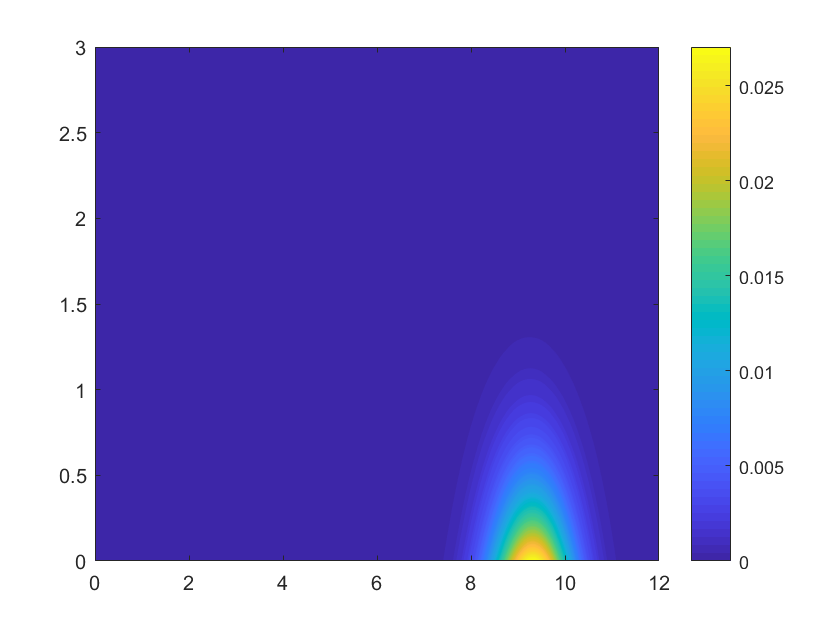
\includegraphics[width=1\textwidth]{t1}
\end{center}
\caption{Oil concentration at time = 1} \label{fig::MyFigure}
\end{figure}

\begin{figure}[bht]
\begin{center}
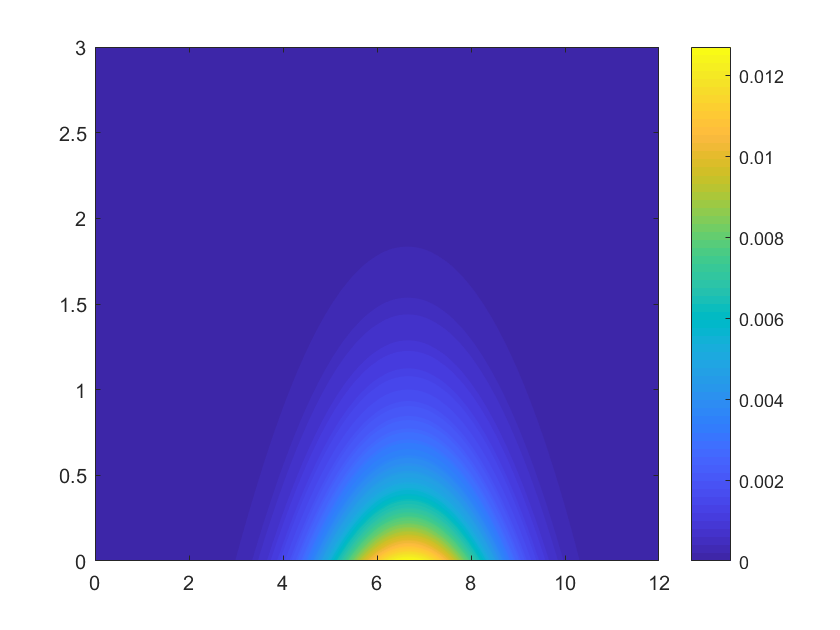
\includegraphics[width=1\textwidth]{t4}
\end{center}
\caption{Oil concentration at time = 4} \label{fig::MyFigure}
\end{figure}

\begin{figure}[bht]
\begin{center}
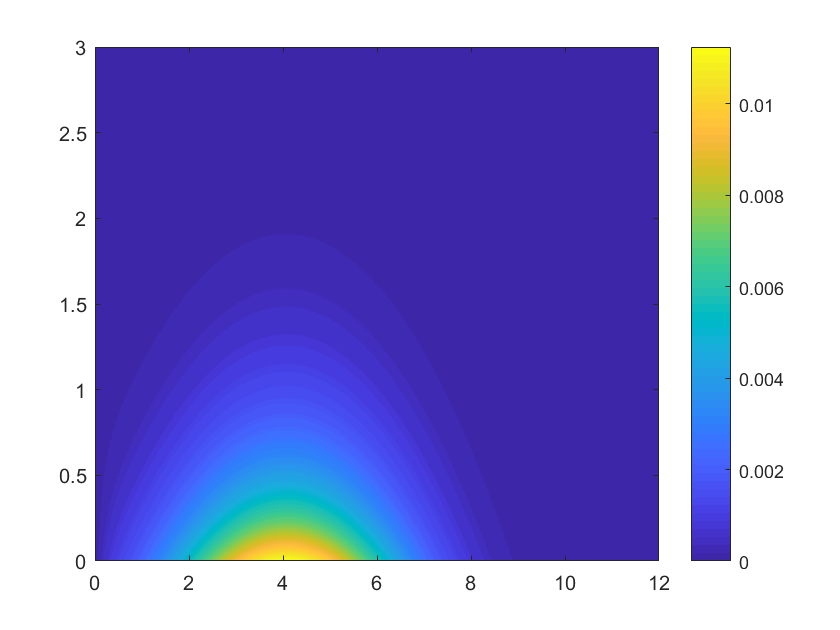
\includegraphics[width=1\textwidth]{t7}
\end{center}
\caption{Oil concentration at time = 7} \label{fig::MyFigure}
\end{figure}

\begin{figure}[bht]
\begin{center}
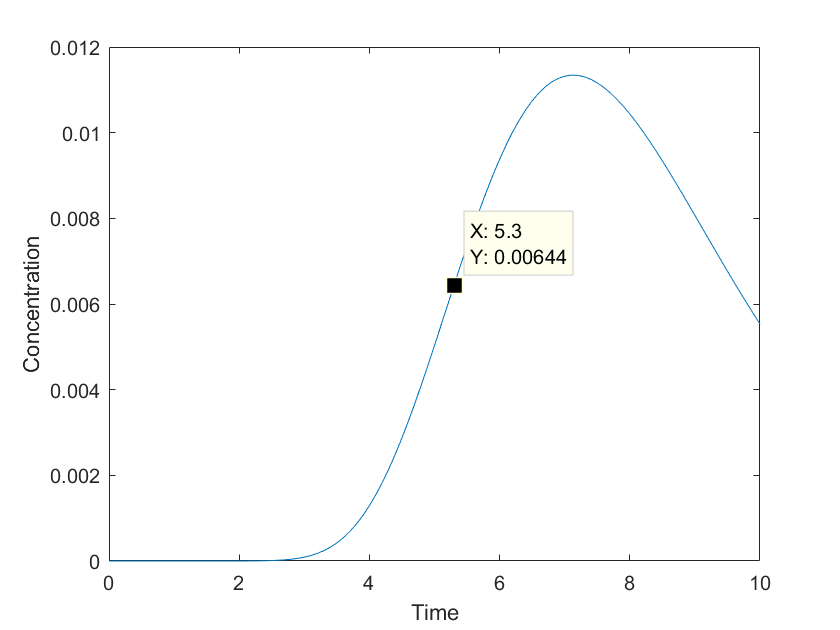
\includegraphics[width=1\textwidth]{concentration4}
\end{center}
\caption{Oil concentration at point (4,0)} \label{fig::MyFigure}
\end{figure}

\begin{figure}[bht]
\begin{center}
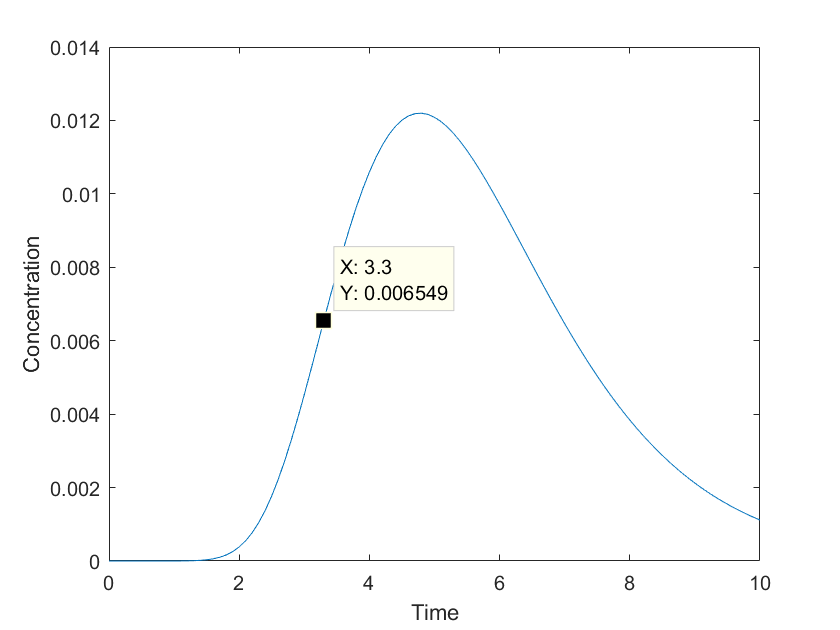
\includegraphics[width=1\textwidth]{concentration6}
\end{center}
\caption{Oil concentration at point (6,0)} \label{fig::MyFigure}
\end{figure}

\begin{figure}[bht]
\begin{center}
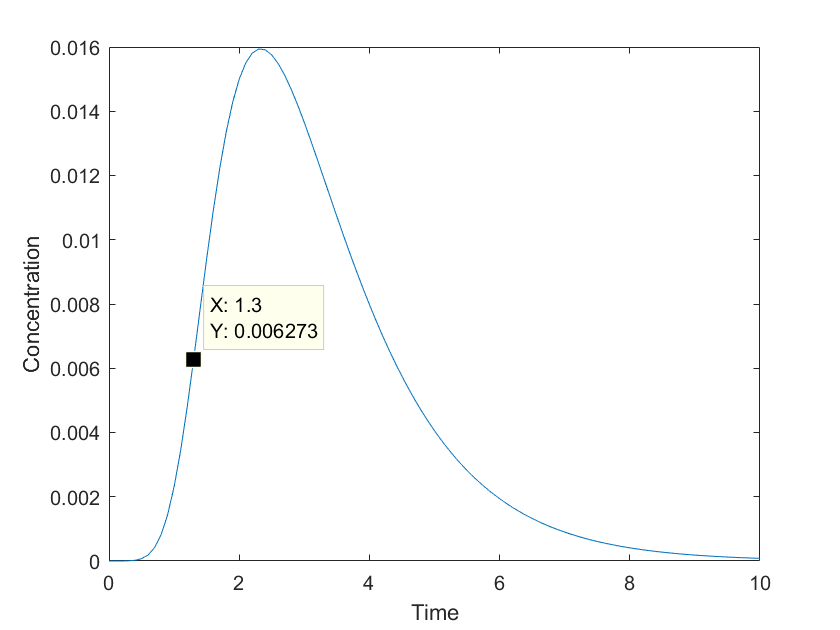
\includegraphics[width=1\textwidth]{concentration8}
\end{center}
\caption{Oil concentration at point (8,0)} \label{fig::MyFigure}
\end{figure}



%%%%%%%%%%%
\newpage
\clearpage
\setcounter{page}{1} \pagestyle{empty}
\section{References}\label{sec::References}
\begin{itemize}
\item [1] Daniil Bochkov, CS 111 - Introduction to Computational Science Lecture 10. Solving Advection Equation 2017
\item [2] Daniil Bochkov, CS 111 - Introduction to Computational Science Lecture 9. Introduction to Partial Differential Equations. 2017
\item [3] Daniil Bochkov, CS 111 - Introduction to Computational Science Final.  2017

\end{itemize}


%%%%%%%%%%%

\end{document}
